% JKAIA 2026 (2026 한국인공지능학회 추계학술대회) -- General (Poster) track
% Template: kaia.cls from the official poster-track zip (202610/4C732AD2...zip, re-downloaded and
% byte-compared 2026-10-24). Poster rule: a 1--2 page summary with title, authors, affiliations and an
% optional abstract. Single-blind, so author names stay in the PDF. Paper in English; the EasyChair
% abstract field is filled in Korean (see ABSTRACT_KO.md).
% Template note: "The Abstract can have 10-20 lines. Do not use symbols, special characters, footnotes,
% or math in Paper Title or Abstract." The abstract below follows that rule.
%
% Workflow: main_ko.tex is the Korean WORKING COPY with the same paragraph structure. The author edits
% the Korean text; the same edits are then applied here, paragraph by paragraph. This file is the SUBMISSION.
% Every number comes from main/results/*.json; paper/build/verify_numbers.py prints each one.
%
% Build:  tectonic -X compile main.tex   (or pdflatex main; bibtex not needed)
%
% Notes on the template (same handling as the DriveWAM poster of the same venue):
%  * kaia.cls \maketitle switches to \twocolumn[...]; the official sample then draws a full-width
%    \fbox{\parbox{\textwidth}{...}}, which cannot break across pages. For a two-page summary we keep
%    the page one-column and draw the same frame with mdframed (page-breakable).
%  * kaia.cls asks for Times via times/mathptmx. Under XeTeX (tectonic) those fonts are not mapped,
%    so we load the system Times New Roman; pdflatex/Overleaf keep the class default.

\documentclass[nouppercase]{kaia}
\usepackage{amsmath}
\usepackage{booktabs}
\usepackage{graphicx}
\usepackage[framemethod=TikZ]{mdframed}
\usepackage{iftex}
\ifXeTeX
  \usepackage{fontspec}
  \setmainfont{Times New Roman}
\fi
\AtBeginDocument{\hypersetup{pdftitle={Near-Miss Blindness: Latent World-Model Imagination Loses Resolution at the Outcome Boundary},pdfauthor={YongHwi Song, Keon Myung Lee}}}
\graphicspath{{../figures/}}

\makeatletter
\renewcommand{\twocolumn}[1][]{#1}   % keep one column; \maketitle's optional argument is still typeset
\@secpenalty=0   % inside mdframed, a negative section penalty made the frame split before C. Algorithms and left page 1 short
\makeatother
\mdfsetup{linewidth=0.4pt, linecolor=black, innerleftmargin=7pt, innerrightmargin=7pt,
          innertopmargin=3pt, innerbottommargin=2pt, skipabove=1pt, skipbelow=1pt}

\title{Near-Miss Blindness: Latent World-Model Imagination Loses Resolution at the Outcome Boundary}

\author{YongHwi Song}{a}
\author{Keon Myung Lee}{b}
\affiliation{School of Information and Communication Engineering, Chungbuk National University, Korea, thddydgnl1937@gmail.com}{a}
\affiliation{School of Software, Chungbuk National University, Korea, kmlee@cbnu.ac.kr}{b}

\begin{document}

\maketitle
\vspace{-34pt}

\begin{mdframed}

\begin{abstract}
Learned world models used to evaluate robot policies have been reported to imagine success for failed executions. We ask which failures are misjudged. We generate counterfactual failures densely around the success boundary, index them by failure distance (task error over success threshold), and judge real and imagined final frames with the same judge to separate judge error from imagination error. Hypotheses, thresholds and decision rules were pre-registered internally (timestamped, hashed design documents). On the public DINO-WM PushT model at a five-step horizon, imagination still separates success from far misses but loses resolution at the boundary: the AUROC of success against near misses falls from 0.953 on real frames to 0.853 in imagination, against far misses only by 0.005, and the near-miss drop grows with the horizon. A probe trained on imagined features reaches only 0.889, so part of the boundary information is lost, and the errors are two-sided rather than optimistic. In a controlled latent model, lowering the training failure rate from 0.3 to 0.03 raises the share of near misses imagined as success from 0.10 to 0.54, all of which is added by imagination, while success misjudgments fall to zero. On the public model a training-free MC dropout discount helps only slightly, and in both latent models boundary-targeted counterfactual data did not outperform simple reweighting. On a video world model the pre-registered boundary-specific hypotheses were not supported, so we limit our claims to the two latent models tested.
\end{abstract}
\begin{keywords}
World models, robot policy evaluation, failure prediction, imagination, pre-registration
\end{keywords}

\subsection{Problem Setup}
World models, from latent planners such as DINO-WM~[1] to video policies such as Cosmos Policy~[2], can evaluate robot policies in imagination: the model rolls out a policy's actions from a real initial observation, and a success judge labels the imagined final frame. Imagination has been reported to predict success for failed executions~[3, 4]. We ask how this error depends on the distance of a failure from the boundary. The failure distance is $r=e/\tau$, the task error over the success threshold (success $r<1$, near-miss $1\le r<2$, far-miss $r\ge 3$). We measure $P(\hat S=1\mid r)$, the success vs.\ near-miss and vs.\ far-miss AUROC on real and imagined frames, the imagination share $(P_{\rm imag}-P_{\rm real})/P_{\rm imag}$ of near-miss misjudgments, and the per-policy over-estimation added by imagination $o^{\rm imag}_\pi$ against the near-miss share $n_\pi$. Models: \textbf{M1}, public DINO-WM PushT; \textbf{M2}, Cosmos Policy on LIBERO~[5]; \textbf{M3}, a controlled DINO-WM-style latent predictor on a rendered 2D pick task, trained with failure rate $p\in\{0.3, 0.1, 0.03\}$.

\subsection{Novelty}
(1) \textit{Boundary-dense failure-distance curves.} CureWM~[3], the closest work, shows optimism of Cosmos Policy and Ctrl-World on counterfactual failures and repairs it with counterfactual fine-tuning, but had too few failures at its severity nearest the boundary and left policy ranking untested; MiraBench~[4] uses one severity. We target $r\in[0.8,3]$ uniformly (over 1,300 near-misses per cell). (2) \textit{Judge vs.\ imagination}: each imagined judgment is paired with the same judge on the real frame, and an imagined-feature probe bounds what remains. (3) \textit{Mechanism}: a dose-response test of success-skewed data; remedies at matched exposure. (4) \textit{Internally pre-registered} hypotheses (primary H1a, H1b, H2a; others exploratory), thresholds, aggregation and go/no-go rules; hashed amendments; negative results reported.

\subsection{Algorithms}
\textbf{Counterfactual failures.} Perturbed actions of successful trajectories cover $r\in[0.8,3]$ evenly plus tails below 0.8 and above 3 (M1: bisection per stratified target, 300 per tail; M2: binned selection, 100 successes and up to 100 far-misses per task; M3: a fixed $r$ grid, far-miss only at its end $r=3$); the simulator gives the true $r$, and the same actions are replayed open-loop in the world model (M1: $H\in\{3,5,7,10\}$ planning steps, 3,600 targets per cell; M2: 4,184 pairs, 6 LIBERO-Goal tasks; M3: 49 values of $r$ $\times$ 128 scenes $\times$ 3 seeds).
\textbf{Judges.} Primary judge (a): an oracle classifier trained on real final frames, used only if its held-out accuracy is at least 0.95 (M1 5-seed ensemble 0.9585, M2 0.974, M3 1.000). Latent goal distance, the Cosmos value head and a VLM are auxiliary.
\textbf{Policies.} M1: 24 Diffusion Policy~[6] checkpoints (3 seeds $\times$ 8 training stages, 100 episodes each); M3: six policies with designed near-miss shares.
\textbf{Remedies.} Boundary-targeted vs.\ full-range (CureWM-style) counterfactuals vs.\ reweighting at matched failure exposure; a training-free MC dropout discount (success only if at least $q^{*}$ of 16 passes agree; $q^{*}$ from a dev set).

\par\smallskip
{\centering
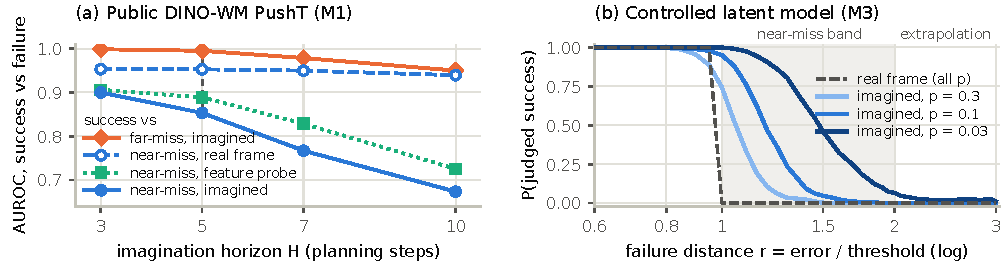
\includegraphics[width=0.85\linewidth]{fig_boundary.pdf}\par
\captionof{figure}{Boundary resolution. (a) M1, validation split, original $r$, judge (a); dashed vertical line: pre-registered cell. (b) M3, frozen judge, 3 seeds pooled; training failures cover only $1\le r<2$.}\label{fig:boundary}\par}
\smallskip

\subsection{Experiments}
{\centering\footnotesize
\setlength{\tabcolsep}{4pt}
\begin{tabular}{lccc}
\toprule
Pre-registered quantity (judge (a), primary cell) & M1 PushT, $H=5$ & M2 LIBERO & M3, $p=0.03$ \\
\midrule
Near-miss judged success: real $\rightarrow$ imagined & 0.112 $\rightarrow$ 0.147 & 0.051 $\rightarrow$ 0.298 & 0.000 $\rightarrow$ 0.535 \\
AUROC drop, success vs.\ near / vs.\ far & 0.100 / 0.005 & 0.275 / 0.137 & 0.107 / 0.000 \\
H1a (near $\ge 0.3$, $\ge 3\times$ far) / H1b (near-specific loss) & no / yes & no / no & yes / 2 of 3 clauses \\
H3: imagination share of near-miss errors $>0.5$ & 0.24, no & 0.83, yes & 1.00, yes \\
H2a: Spearman$(n_\pi, o^{\rm imag}_\pi)\ge 0.6$ & 0.36, no & not run & 0.83, yes \\
\bottomrule
\end{tabular}\par
\captionof{table}{Pre-registered tests. The primary hypotheses H1a, H1b and H2a each hold in one model only and fail the two-model rule; the exploratory H3 holds in M2 (with a judge caveat) and M3.}\label{tab:tests}\par}
\smallskip

\textbf{Boundary loss on a public latent model (M1).} At $H=5$ the success vs.\ near-miss AUROC drops by 0.100 [95\% CI 0.075, 0.125] and the success vs.\ far-miss AUROC by only 0.005 [0.001, 0.010]; the near-miss drop grows by 0.031 [0.025, 0.039] per unit of $H$ (Fig.~\ref{fig:boundary}a). The specificity is limited: far-misses also blur beyond $H=5$ (0.021, 0.048) and at every $H$ under the object-pose error definition (0.058--0.129). The imagined-feature probe reaches 0.889 (drop 0.064 [0.046, 0.084]), so part of the loss is in the information itself. The errors are two-sided: successes are judged successful less often (0.862 to 0.710) and near-misses more often (0.112 to 0.147).
\textbf{Success-skewed data converts the blur into optimism (M3; exploratory H4a).} As $p$ falls from 0.3 to 0.1 to 0.03, near-miss misjudgment rises from 0.10 to 0.24 to 0.54 and success misjudgment falls from 0.021 to 0.005 to 0.000 ($p=0.03$ vs.\ 0.3: $+0.431$ [0.406, 0.457] and $-0.021$ [$-0.030$, $-0.014$]; Fig.~\ref{fig:boundary}b). A perfect real-frame judge and an imagined-feature probe at 0.986 show that this error is mainly a shift toward success rather than a loss of information. Imagined over-estimation follows the near-miss share (Spearman 0.83 [0.77, 0.94] with the share taken on $1\le r<1.2$, fixed before analysis; 0.66 on $1\le r<2$): policies with real success 0.48--0.53 are imagined at 0.58, 0.72 and 0.99, but their ordering is preserved. M1 gives a partial result: a short (3,000-step) success-skewed fine-tuning lowered only success misjudgment (near-miss misjudgment rose only under the object-pose definition), and the 24 checkpoints' $o^{\rm imag}_\pi$ stays within $-0.01$ to $+0.06$.
\textbf{Remedies (exploratory).} At matched exposure, boundary-targeted counterfactuals did not outperform reweighting in any of the 3 settings (worse on M3 by 0.040 and 0.046), so we do not propose them. On M1, the MC dropout discount lowers mean absolute policy bias from 0.0233 to 0.0187 ($-0.0046$ [$-0.0088$, $-0.0004$]) and a failure-geometry-weighted rank error from 0.0225 to 0.0171, a small gain, since M1's bias is itself small.
\textbf{Video world model.} On M2, far-misses blur along with near-misses (no boundary-specific pattern); imagination adds most of its near-miss errors (0.051 to 0.298), though part of this share may come from its real-frame judge, whose operating point shifts on imagined frames. \textbf{Capacity} (not pre-registered): M3's near-miss misjudgment is 1.000, 0.535 and 0.149 for small, default and large predictors.

\par\vspace{1pt}\noindent{\scriptsize\textbf{References.}
[1]~G.~Zhou, H.~Pan, Y.~LeCun, L.~Pinto, DINO-WM, arXiv:2411.04983, 2024.
[2]~M.~J.~Kim et al., Cosmos Policy, arXiv:2601.16163, 2026.
[3]~J.~Xu et al., CureWM, arXiv:2610.09134, 2026.
[4]~T.~Yang et al., MiraBench, arXiv:2605.29360, 2026.
[5]~B.~Liu et al., LIBERO, NeurIPS Datasets and Benchmarks, 2023.
[6]~C.~Chi et al., Diffusion Policy, RSS, 2023.\par}

\end{mdframed}

\end{document}
